\chapter{Algoritmos Genéticos\label{cap:ga}}

Da-se o nome \emph{Algoritmos Genéticos} (GAs) a uma técnica de busca baseada numa metáfora da Evolução. Na Natureza muitos animais competem entre si por recursos limitados, e os vencedores de uma dada população têm mais change de procriação. Seu êxito vem das catacterísticas que os tornam melhor adaptados para os desafios apresentados pelo ambiente onde vivem. Seus filhos levarão essas características adiante. 

Esse mecanismo de seleção dos melhores foi descoberto por Darwin, que o chamou de Seleção Natural. A partir dele foi possível explicar como a natureza gera organismos complexos e capazes de solucionar problemas difíceis. Darwin não sabia como as características eram transmitidas e como novas surgiam.

Fazendo experimentos com plantas, Mendel determinou como se dá a transmissão. Há uma unidade básica de informação associada às características dos organismos, que ele chamou de Gene. Definiu como \emph{Fenótipo} as características externas de um organismo, e \emph{Genótipo} o conjunto de genes associados a um dado fenótipo. Na reprodução sexuada os filhos possuem uma mistura entre os genes do pai e da mãe. Por isso, não são idênticos a nenhum dos seus progenitores, mas são semelhantes a eles.

Sabe-se hoje que toda a informação de um organismo está codificada no DNA, que contém os genes. A combinação entre os genes dos pais acontece durante a reprodução, num evento chamado de Cruzamento Cromossômico, ou \emph{Crossing$-$Over}, onde há troca de informação entre os cromossomos. Durante a cópia do DNA ocorrem, com baixíssima probabilidade, erros eventuais, fazendo com que o filho tenha um novo atributo. 

Se a nova característica for muito boa, após várias gerações ela estará espalhada por toda população. O indivíduo será beneficiado na competição e provavelmente se reproduzirá mais, assim como seus filhos. A cada nova geração, mais indivíduos possuirão o novo fenótipo, perpetuando a transmissão dos genes assossiados. 

Apesar de não ter sido o primeiro a utilizar ideias da Evolução em Ciência da Computação, John Holland é considerado o pai dos Algoritmos Genéticos. Ele estudou formalmente, do ponto de vista matemático, a adaptação na natureza e propôs uma heurística baseada nesse estudo. Seu objetivo era simular a Evolução em computadores. Em 1975 publicou o livro \emph{Adaptation in Natural and Artificial Systems}. A partir de então muitos passaram a usar GAs na solução de problemas de diversas áreas.

O algoritmo genético mais básico é composto por cinco processos (figura \ref{fig:fluxoGABasico})

\begin{itemize}

	\item \textbf{Gerar população inicial}: População inicial gerada aleatoriamente.
	
	\item \textbf{Avaliação}: Cada indivíduo recebe uma nota. Maiores notas indicam indivíduos mais aptos (soluções mais próximas do objetivo). Esta medida é conhecida como \textit{Fitness}. 
	
	\item \textbf{Teste do critério de parada}: Com todos os indivíduos avaliados, é possível verificar se algum deles representa uma boa solução.
 
	\item \textbf{Seleção}: A Seleção escolhe os sobreviventes da população atual que comporão a próxima população. Um bom processo de seleção atribui maior chance aos indivíduos com melhores \emph{fitness}.
 
	\item \textbf{Reprodução (\emph{crossover})}: Com probabilidade alta (\approx 70\%), indivíduos são selecionados aleatoriamente e geram filhos através da combinação de seus genes.
	
	\item \textbf{Mutação}: Com baixíssima probabilidade (\approx 1\%), genes são escolhidos para sofrer alterações em seus valores.
	
\end{itemize} 

\begin{figure}[htbp]
	\centering
		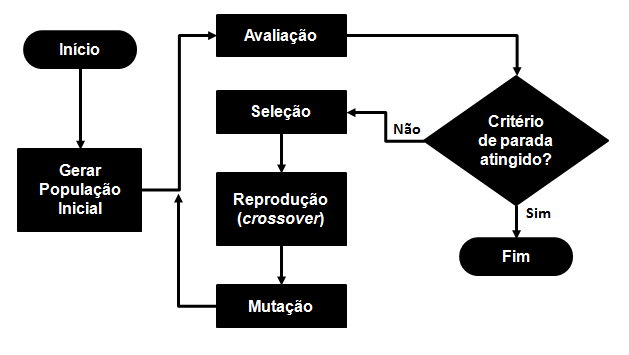
\includegraphics[width=1.00\textwidth]{figs/ga/fluxoGABasico.png}
	\caption{Fluxograma do algoritmo genético típico.}
	\label{fig:fluxoGABasico}
\end{figure}

$----------------------------------------$

\section{Principais Elementos de um Algoritmo Genético}
	
	\subsection{Representação Cromossomial}

	O cromossomo é uma cadeia de caracteres (genes) de comprimento \textit{L}, que representa um indivíduo candidato a solução do problema proposto.
	
	Esta representação compreende parte de grande importância num GA, pois é a partir desta estrutura que os indivíduos serão avaliados e também sofrerão a atuação dos operadores de variação (\textit{crossover} e mutação) e seleção. Uma boa codificação do cromossomo influi diretamente no sucesso da aplicação de um GA.
	
	No momento da definição desta representação, deve-se ter em mente \cite{Linden2008}:
	
	\begin{itemize}
\item Deve ser a mais simples possível.
\item Soluções proibidas não devem ser representadas. 
\item Condições de qualquer tipo devem estar implícitas na representação.
\end{itemize} 
	
	A representação binária introduzida por Holland \cite{Holland} é a mais comum entre os GAs, por facilitar a utilização dos operadores genéticos e ser de fácil manipulação.
	
	Caso se faça necessário, um cromossomo pode conter mais de uma variável em sua cadeia, sendo que estas serão concatenadas para representar o indivíduo. Na tabela \ref{tabCromo} é exibido um exemplo com três possíveis indivíduos com cromossomo multivariável (variáveis x1 e x2) de comprimento $L = 5$ e alelos que variam entre 1 e 0. Porém, é possível implementar soluções com \textit{k} diferentes alelos para cada locus do cromossomo, contudo a dificuldade em manipular esta estrutura será maximizada.
	
	Os exemplos dessa seção utilizam representação binária. Mas pode-se utilizar outros tipos de representação. Decimal, inteira, símbolos etc. Isso faz do GA importante ferramenta para a vida real.
		
	\begin{table}[htp]
 \caption{\label{tabCromo}Exemplo de representação cromossomial}
 \begin{center}
  \begin{tabular}{c|c|c}
   \hline
   Indivíduo & x1  & x2 \\
   \hline
   1 & 10010    & 01101 \\
   2 & 00110    & 11100 \\
   3 & 11101		& 01001 \\ 
   \hline
   \end{tabular}
 \end{center}
\end{table}

%========================TIAGO - fim ========================================================
	
	\subsection{Função de Avaliação}
	
	Na Introdução foi dito que a função de avaliação tem um papel fundamental em um algoritmo genético. Podemos ir além, afirmando que ela é o elo mais forte - senão o único - entre o algoritmo e o problema que tentamos resolver no mundo real. Aliás, geralmente a principal diferença entre dois GAs reside apenas, e justamente, na função de avaliação. Portanto, não seria estranho concluir que ela deve conter todo o conhecimento do problema, incluindo suas condições e restrições.
	
	Mas, afinal, o que \textit{é} a função de avaliação? Uma vez definido o problema e, em seguida, o objetivo do algoritmo, ela representa nesse contexto a qualidade de um indivíduo. Em outras palavras, através da função de avaliação devemos ser capazes de identificar se um cromossomo leva ou não à uma boa solução. Assim, ela deve refletir a meta que desejamos atingir.
	
	Ao aplicarmos a função de avaliação\footnote{Essa função também pode ser chamada de Função Custo, por isso o $f_c$ na equação \ref{funcaval}.} em um indivíduo obtemos uma nota associada aquele cromossomo. Essa nota é um número, um escalar, que pode ser discreto (inteiro) ou contínuo (real):
	
	\begin{equation}\label{funcaval}
		n = f_c(cromossomo)
	\end{equation}
	
	Então, já podemos apresentar a primeira característica de uma função de avaliação: quanto maior a nota, melhor o indivíduo. Pensando em termos da Teoria da Evolução, maiores notas exprimem indivíduos mais adaptados ao ambiente (metas). Além disso, na equação \ref{funcaval}, $n$ é uma métrica que deve identificar o quão próximo um cromossomo está de uma boa solução.
	
	Por exemplo, suponha que o cromossomo $c_1$ tem nota $n_1 = 10$, enquanto $n_2 = 9,7$ é atribuída ao cromossomo $c_2$. Imaginando hipoteticamente que uma boa solução está próxima de $n_{boa} = 11$, podemos concluir que ambos são bons, mas $c_1$ é melhor. Sintetizando, uma boa função de avaliação deve quantificar, dentre boas soluções, quais são as melhores.
	
	Outro número importante é o \textit{fitness} médio ($<n>$), ou seja, a razão entre a soma das notas de todos os indivíduos e o número de indivídios na geração ($N$):
	
	\begin{equation}\label{fitness_medio}
		<n> = \frac{\sum_{i = 1}^{N} n_i}{N}
	\end{equation}
	
	
	Quando não sabemos qual será a maior nota possível para o nosso problema, temos a opção de usar a estabilidade de $<n>$ como critério de parada. Por quê? Porque se a média das notas não muda muito com o passar do tempo, podemos concluir que o material genético disponível indivíduo a indivíduo é muito semelhante, e essa ausência de variabilidade faz com que uma geração futura se pareça com a passada. Em linguagem mais técnica, estamos confinados a uma região específica no espaço de soluções.
	
	Com relação ao comportamento da função de avaliação, É extremamente desejável que  seja suave e regular. O que isso quer dizer? Que, se um indivíduo é levemente superior a outro, sua nota deve ser apenas um pouco maior. Infelizmente, na maioria das vezes isso não acontece, e o impacto pode surgir em forma de instabilidade do \textit{fitness} médio. Na figura \ref{figFitness} encontramos dois exemplos.

	\begin{figure}[htp]
		\begin{center}
			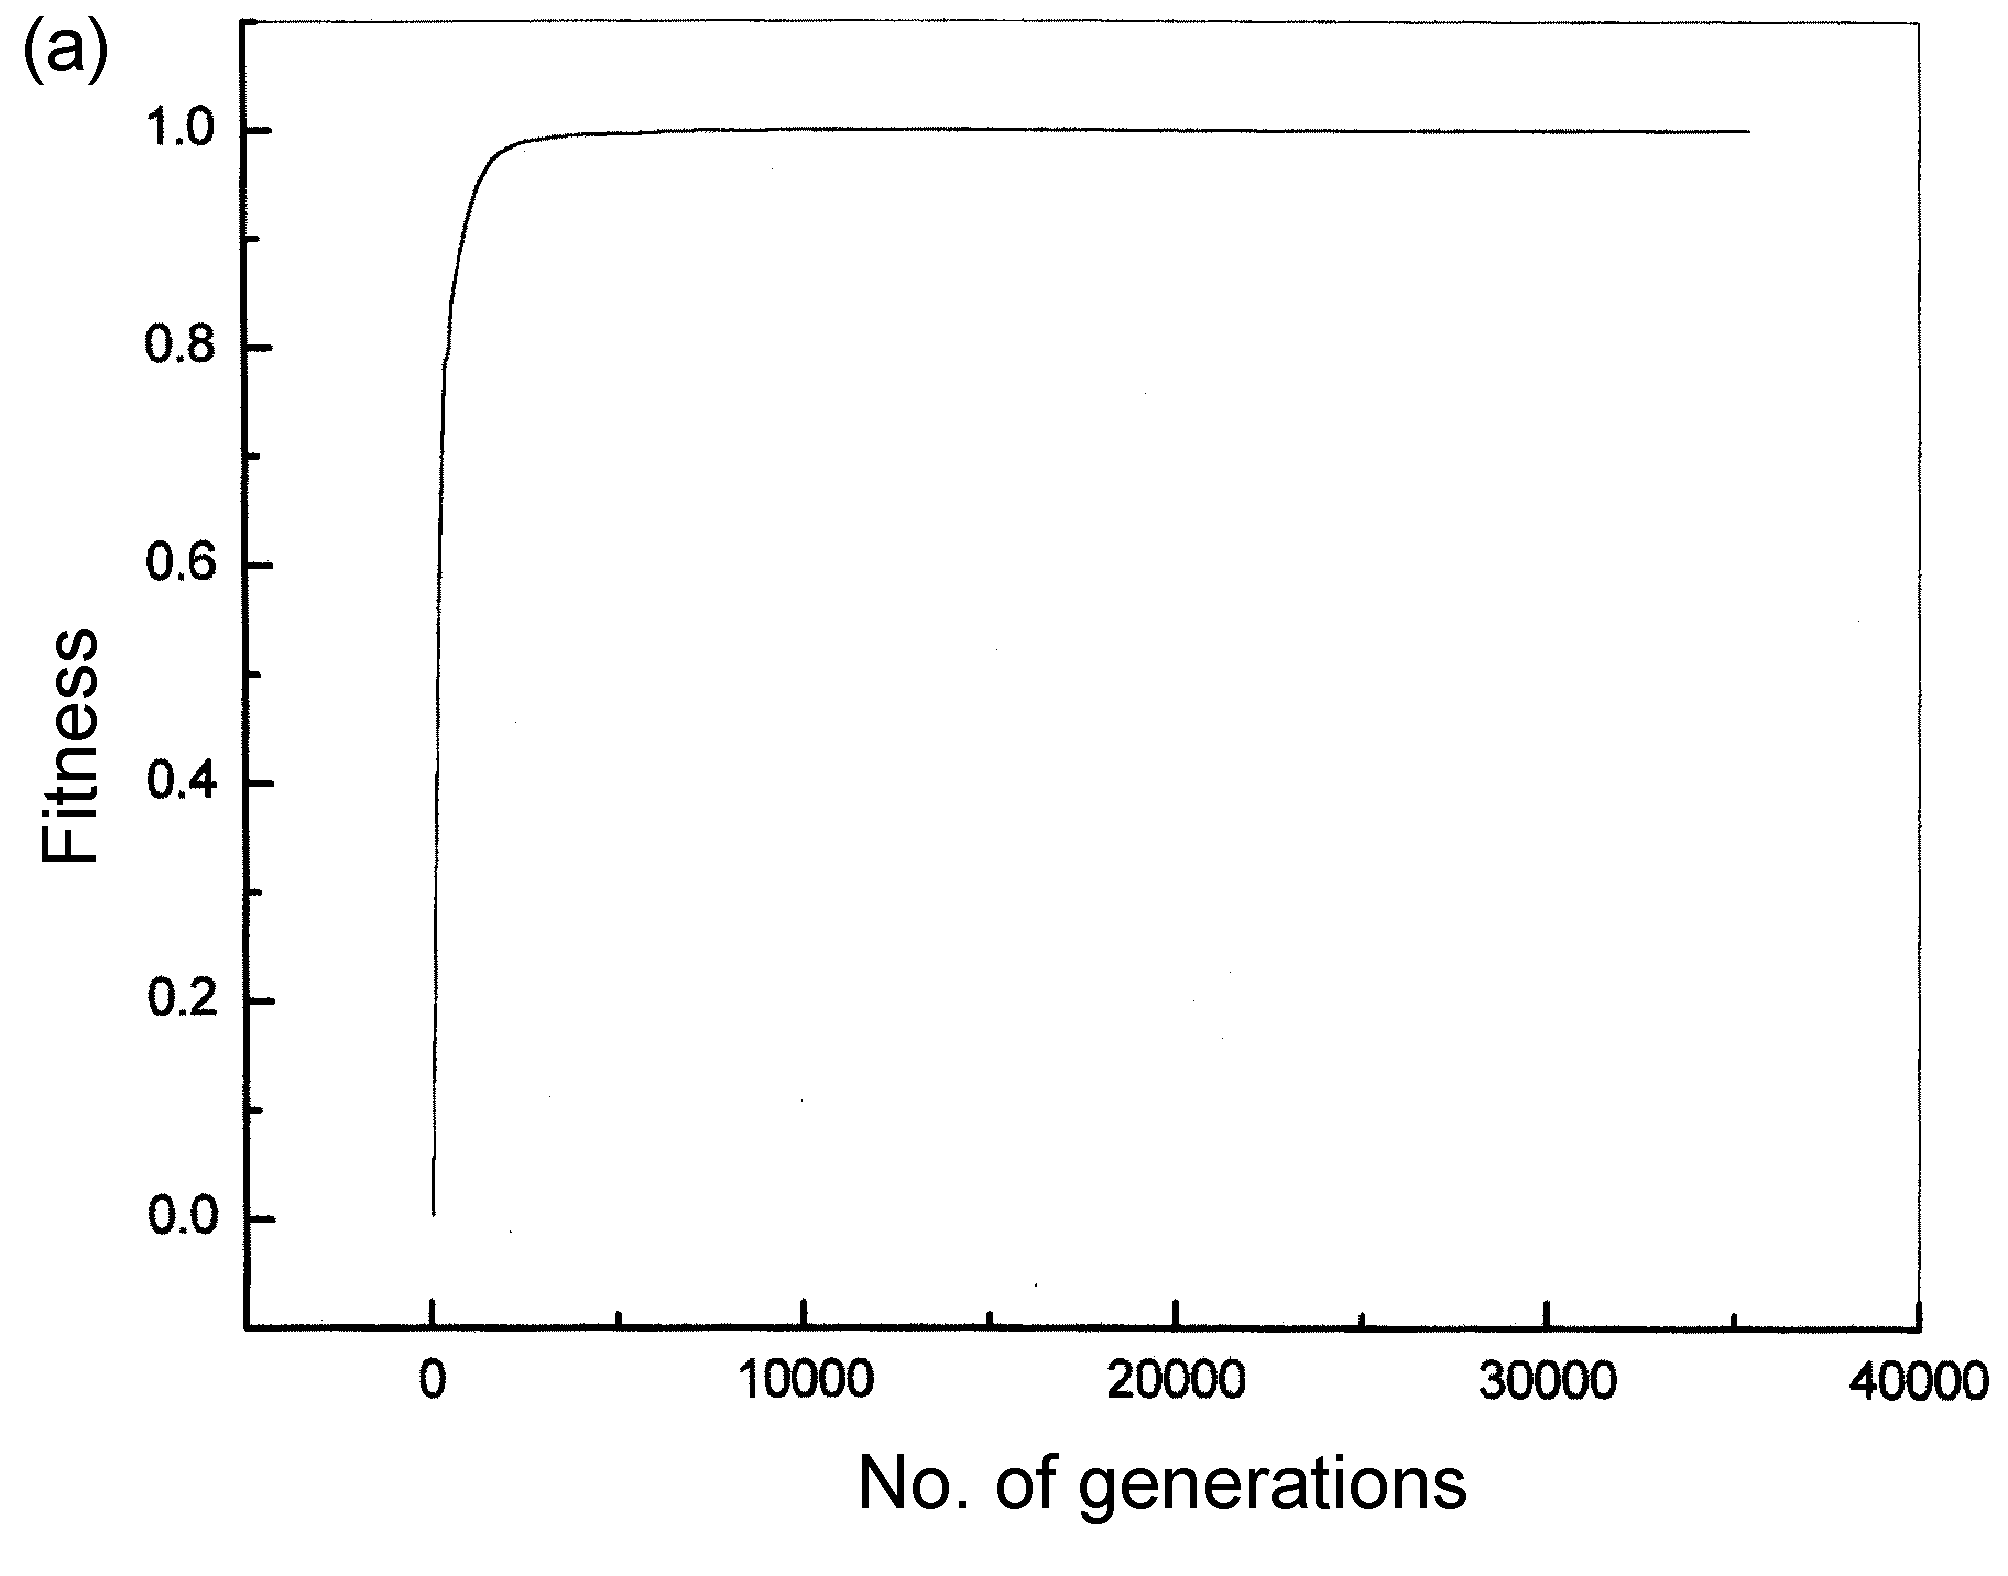
\includegraphics[height=4.7cm]{figs/ga/func_aval_estavel.png}
			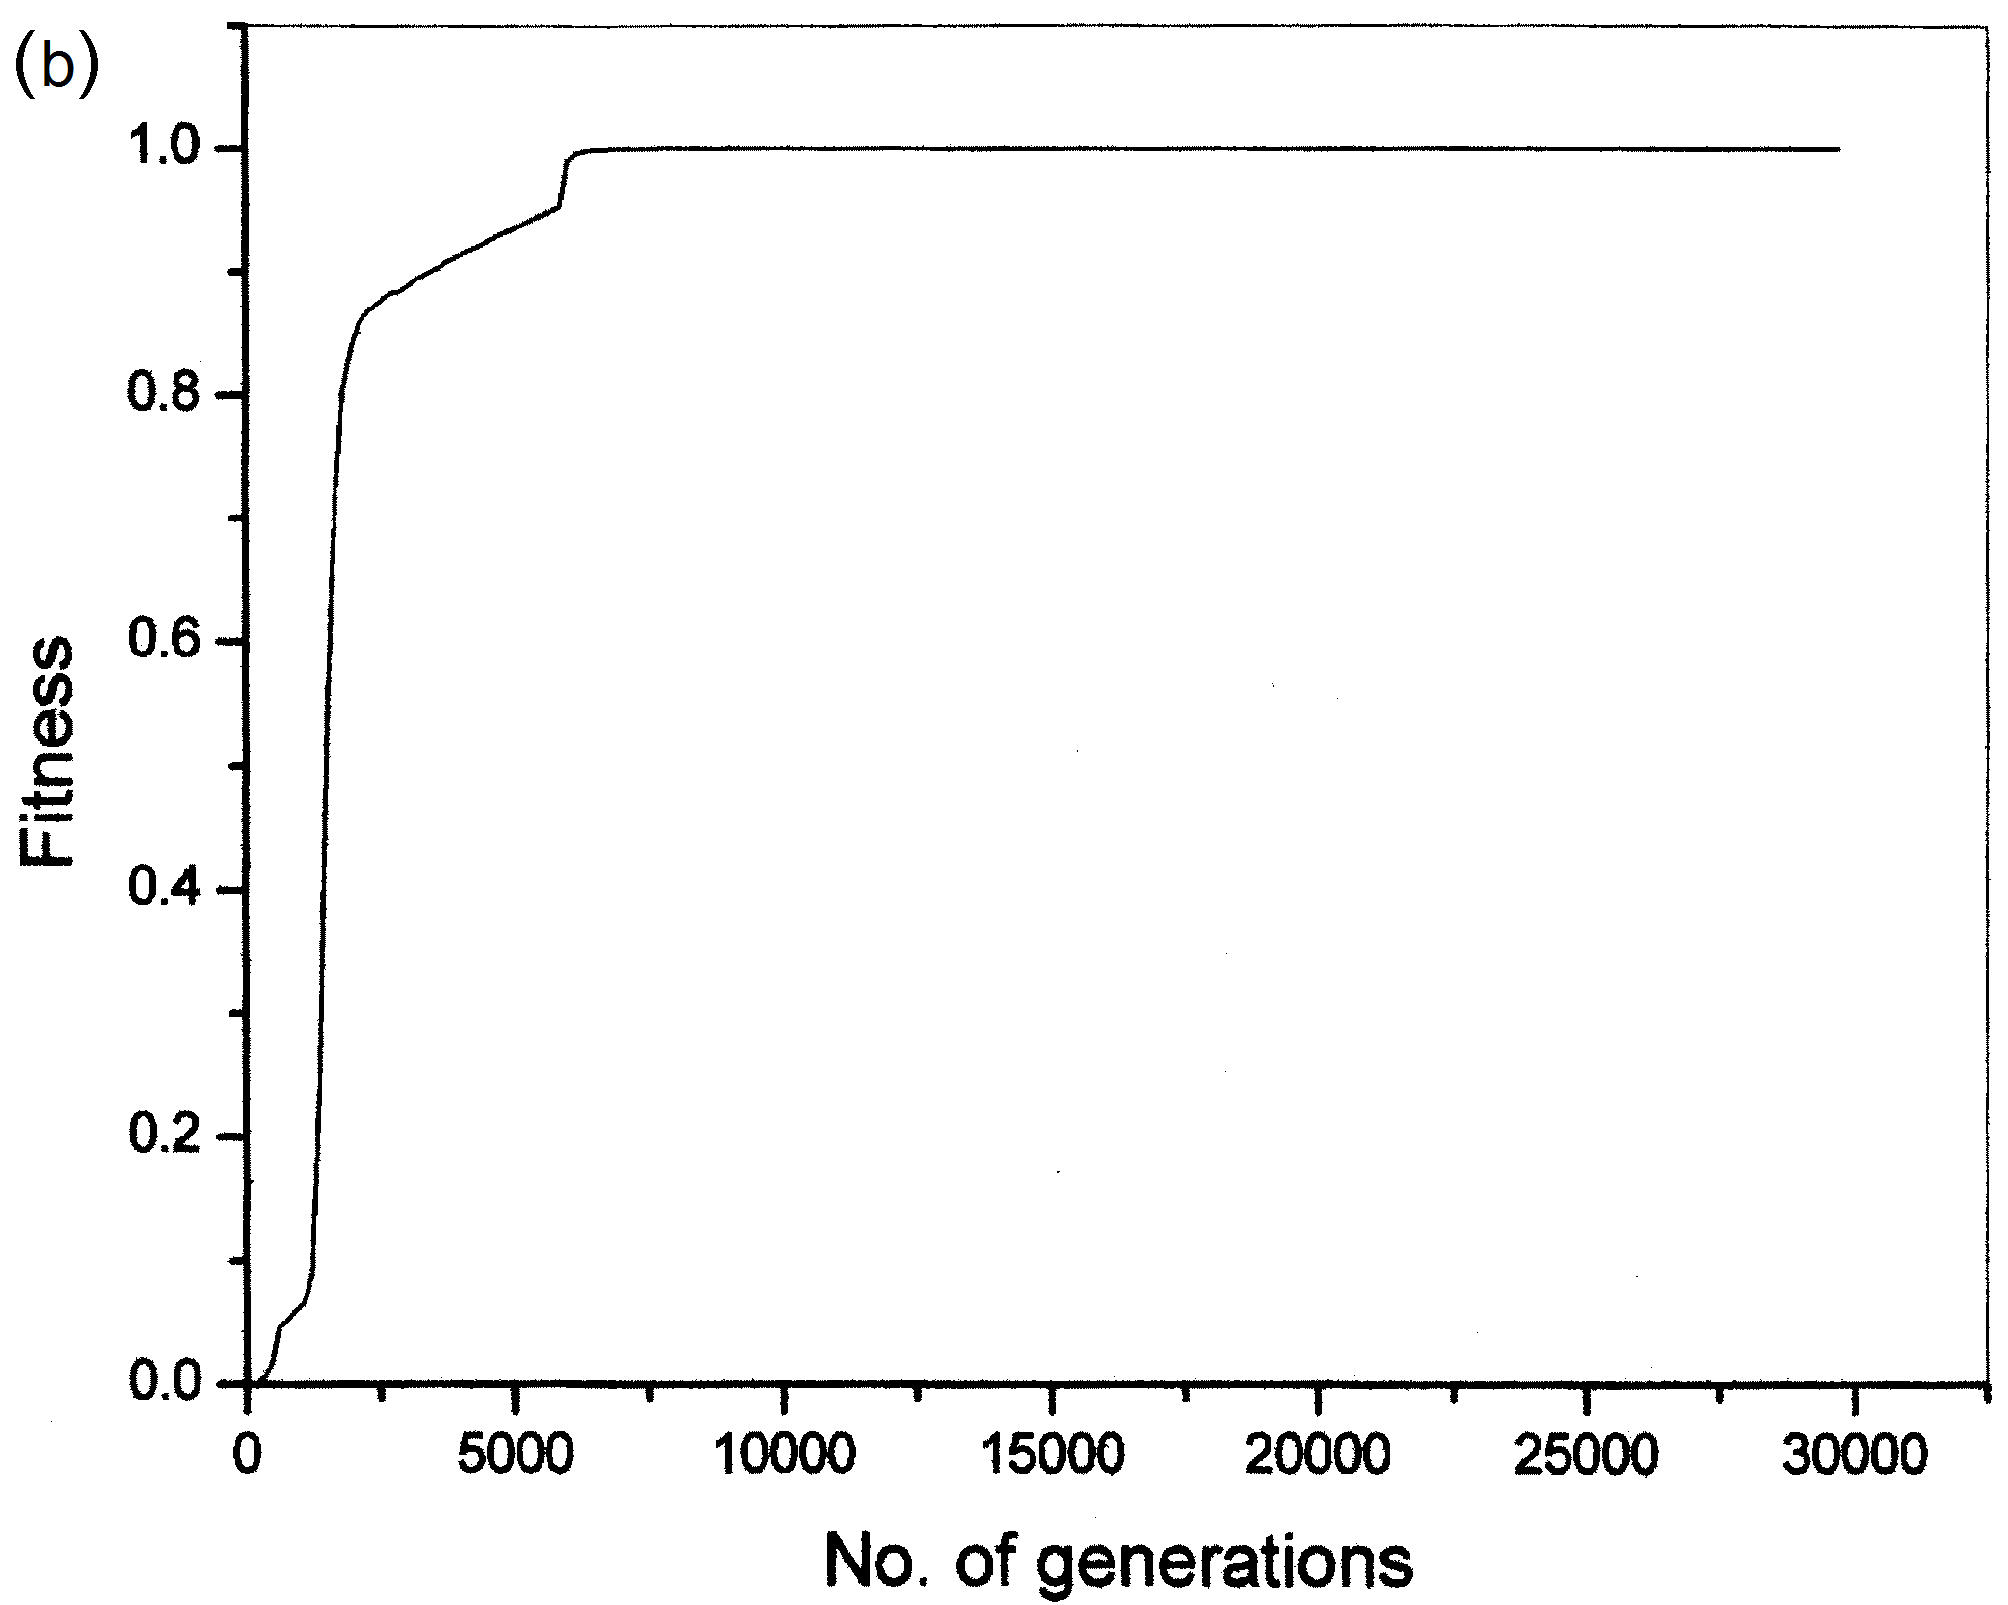
\includegraphics[height=4.7cm]{figs/ga/func_aval_instavel.png}
		\end{center}
		\caption{\label{figFitness}Exemplo de instabilidade do \textit{fitness}. Enquanto em (a) o \textit{fitness} cresce de maneira contínua e depois se estabiliza, em (b) há alguns pontos onde onde o comportamento da nota sofre uma mudança razoavelmente brusca. Gráficos retirados de \cite{Bhattacharyya2004}.}
	\end{figure}

	Na próxima seção discutiremos um exemplo de definição de uma função de avaliação.
		
	\subsection{\label{MaxSeno}Exemplo: Máximos de $f(x) = \sin(x) / x$}
	
	A função
	
	\begin{equation}\label{eqSinX}
		f(x) = \frac{\sin(x)}{x}
	\end{equation}
	aparece em várias áreas da matemática. Seu caráter oscilatório é muito útil para descrever pacotes de onda na mecânica quântica \cite{QuGA2006} ou auxiliar no estudo das transformadas de Fourier \cite{James2002}.
	
	\begin{figure}[htp]
		\begin{center}
			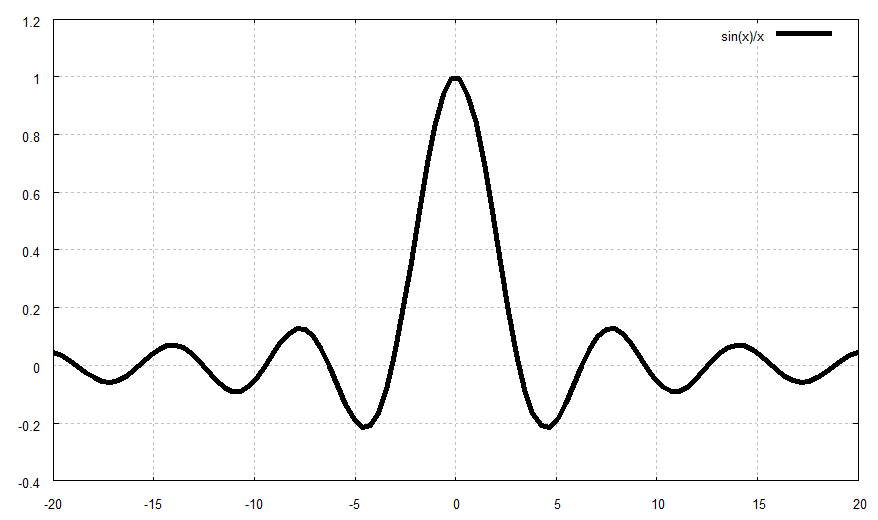
\includegraphics[width=13cm]{figs/ga/sen_x__x.png}
		\end{center}
		\caption{\label{figSen}Gráfico da função $f(x) = \sin(x) / x$ para $x = [-20,20]$. Se desejamos encontrar os máximos (global ou locais), uma boa função de avaliação seria a própria $f(x)$. Gráfico gerado com o GnuPlot \cite{gnuplot}.}
	\end{figure}
	
	Observando seu gráfico na figura \ref{figSen}, vemos que ela tem um máximo global em $x = 0$ e vários máximos locais. Imaginando que quiséssemos obter os valores de $x$ onde esses máximos aparecem, como definir uma boa função de avaliação?
	
	Nesse caso podemos utilizar a própria $f(x)$ (equação \ref{eqSinX}), pois ela possui boas características. Pelo gráfico \ref{figSen} concluímos que ela é suave e, se compararmos dois valores bem próximos de $x$, o resultado de $f(x)$ também é. Por exemplo, $f(0,5) = 0,9589$ e $f(0,51) = 0,9572$, evidenciando que o ponto $x = 0,5$ é um indivíduo levemente melhor.
	
	
	\begin{table}[htp]		
		\caption{\label{tabSen}Valores de $x$ gerados aleatoriamente para a função $f(x) = \sin(x)/x$. A própria $f(x)$ pode ser usada como função de avaliação.}
		\begin{center}
			\begin{tabular}{c|c|c}
				\hline
				\textbf{Indivíduo}& $\textbf{x}$		& $\textbf{f(x)}$ \\
				\hline
				01 & 	2							& 0,455 \\
				02 & 	3							& 0,047 \\
				03 &	-9						& 0,046\\	
				04 &	-8							& 0,124 \\
				05 &	19							& 	0,008 \\
				\hline
				\multicolumn{2}{r}{\textbf{Soma:}} & 0,680 \\
				\hline
			\end{tabular}
		\end{center}
	\end{table}
	
	
	Se escolhermos vários valores para $x$ aleatoriamente, basta aplicar a $f(x)$ e selecionar os maiores\footnote{Em geral deve-se impor algumas restrições na função de avaliação. Veremos na seção \ref{selecao} que valores negativos são proibidos para o método da Roleta.}. Na tabela \ref{tabSen} listamos cinco pontos como exemplo, assim como a soma dos resultados de $f(x)$. Como veremos na próxima seção, os pontos $01$ e $04$ têm, respectivamente, $0,455/0,680 = 66,9\%$ e $ 0,124/0,680 = 18,2\%$ de chance de serem selecionados no processo de Seleção.
	
	\subsection{\label{selecao}Seleção}
	
	A parte do algoritmo genético que chamamos de \textit{Seleção}\footnote{Alguns autores chamam esse módulo de Seleção de Pais, enquanto outros o definem exatamente como na biologia, Seleção Natural. Para evitar mal entendidos, optamos por chamá-lo apenas de Seleção.} tem como objetivo simular o processo de Seleção Natural da Evolução. Basicamente, os  mais aptos, leia-se ``com maior \textit{fitness}'', devem gerar mais descendentes.
	
	Porém, exatamente como na natureza, os indivíduos avaliados com notas menores não devem ser totalmente descartados, e há bons motivos para isso. Em primeiro lugar, esses cromossomos, apesar de mal avaliados, podem conter informação genética importante, senão fundamental, para uma boa solução. Em segundo, a seleção apenas dos melhores, chamada de Elitismo \cite{Bhattacharyya2004}, pode levar à uma convergência precose e com soluções não tão boas.
	
	\subsubsection{\label{ExemploVariabilidade}Exemplo: Variabilidade Genética}
	
	Como exemplo da importância da variabilidade genética, imagine o problema de encontrar o valor máximo da função $f(x) = -x^2 + 36$ no intervalo (discreto) $x = [0,7]$. Assim, uma representação cromossomial binária com 3 \textit{bits} é suficiente, pois 0 = 000 e 7 = 111 (tabela \ref{tabRepCroX2}).
	
	\begin{table}[htp]
 		\caption{\label{tabRepCroX2}Representação cromossomial para os pontos $x = 0$ até $x = 7$ dentro do problema de máximo da função $f(x) = -x^2 + 36$.}
 		\begin{center}
  		\begin{tabular}{c|c}
   			\hline
   			\textbf{x (decimal)}  & \textbf{x (representação binária)} \\
   			\hline
   			0 & 000 \\
   			1 & 001 \\
   			2 & 010 \\ 
   			3 & 011 \\
   			4 & 100 \\
   			5 & 101 \\ 
   			6 & 110 \\
   			7 & 111	\\
   			\hline
   		\end{tabular}
 		\end{center}
	\end{table}
	
	\begin{figure}[htp]
		\begin{center}
			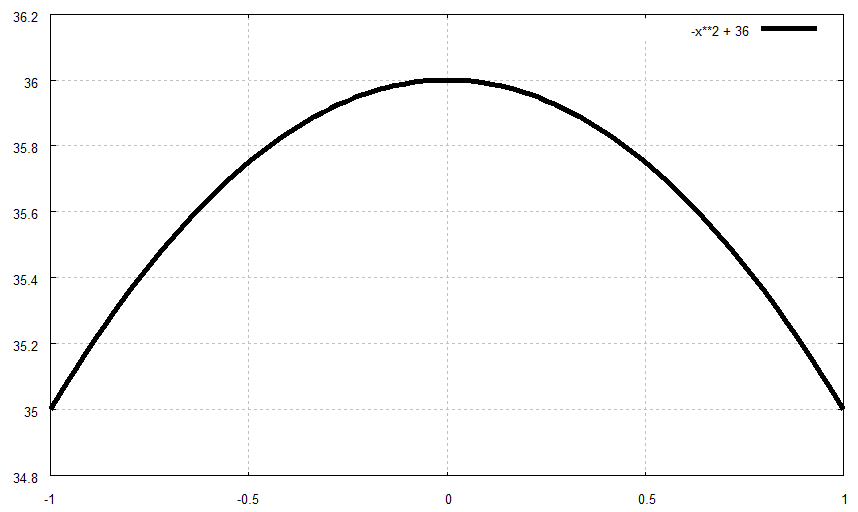
\includegraphics[width=13cm]{figs/ga/Parabola.png}
		\end{center}
		\caption{\label{figParabola}Gráfico da função $f(x) = -x^2 + 36$ para $x = [-1,1]$. Gráfico gerado com o GnuPlot \cite{gnuplot}.}
	\end{figure}
	
	 Vemos na figura \ref{figParabola} que a resposta correta é $x = 0$, cujo valor é $f(0) = 36$. Suponha agora que os dados da tabela \ref{tabFuncMax} representem a população inicial do algoritmo. Se escolhêssemos apenas os indivíduos com as melhores notas, ou seja, $x = 2$ e $x = 3$, descartaríamos o indivíduo $x = 5$ e perderíamos uma importante característica genética: o zero no \textit{bit} central.
	 
\begin{table}[htp]
		\caption{\label{tabFuncMax}População inicial para o problema de máximo da função $f(x) = -x^2 + 36$. O valor de máximo ocorre em x = 0, ou x = 000 na representação binária.}
		\begin{center}
			\begin{tabular}{c|c}
				\hline
				$\textbf{x}$ (decimal)		& $\textbf{x}$ (binário) \\
				\hline
				2							& 010 \\
				7							& 111 \\
				5							& 101 \\	
				3							& 011 \\
				\hline
			\end{tabular}
		\end{center}
	\end{table}
		
		O que aconteceria depois? O mais próximo do valor máximo que o algoritmo conseguiria chegar seria $f(2) = 32$, independentemente do \textit{crossover} entre os indivíduos restantes. Portanto, esse resultado final seria considerado prematuro, efeito denominado \textbf{Convergência Genética}. Em outras palavras, se apenas os melhores indivíduos se reproduzirem, as novas gerações chegarão rapidamente a um estado em que os cromossomos são muito semelhantes entre si, minando a diversidade genética e impedindo a evolução de prosseguir satisfatoriamente.
		
		Vários métodos foram criados para executar a Seleção de maneira coerente, ou seja, privilegiando os indivíduos com alta função de avaliação, mas não desprezando totalmente os de menor nota. O método mais utilizado em aplicações de Algoritmos Genéticos é o da Roleta, assunto da próxima seção.
	
	\subsubsection{O método da Roleta (\textit{Roulette Wheel})}
	
	A ideia do método é simular uma roleta parecida com as utilizadas em cassinos. Entretando, há duas diferenças. Enquanto na roleta tradicional temos o mesmo tamanho de fatia para cada número, na roleta para os algoritmos genéticos a fatia que cada indivíduo ganha é proporcional à sua avaliação.
	
	Uma vez calculados os ângulos para cada cromossomo, giramos a roleta e selecionamos o indivíduo. Nesse ponto reside a segunda diferença. Nos cassinos, o número é selecionado por uma bolinha que também está em movimento. Já nos algoritmos genéticos, o cromossomo é selecionado por um marcador fixo em uma roleta que lembra a utilizada no jogo \textit{Roda a Roda} do SBT \cite{roda-a-roda}.
	
	Na tabela \ref{tabSumFitness} temos os valores dessas fatias (em porcentagem e graus) para o exemplo da seção \ref{ExemploVariabilidade}. Note que o indivíduo 2 foi descartado, e esse é um ponto muito importante no método da roleta. \textbf{indivíduos com avaliações negativas não podem ocupar a roleta}, e o motivo é simples: notas negativas levam a pedaços negativos na roleta, como, por exemplo, - 15\% ou -125$^\circ$.
		
	\begin{table}[htp]		
		\caption{\label{tabSumFitness}Todas as notas dos indivíduos para o exemplo da seção \ref{ExemploVariabilidade}. Lembre-se que para obter máximo da função $f(x) = -x^2 + 36$ podemos utilizar, com algumas restrições, a própria $f(x)$ como função de avaliação $f_c(x)$ (seção \ref{MaxSeno}).}
		\begin{center}
			\begin{tabular}{c|c|c|c|c|c}
				\hline
				\textbf{Indivíduo}	& $\textbf{x}$		& $\textbf{f(x)}$	& \textbf{f$_c$(Indivíduo)} & \textbf{Ocupação (\%)} & \textbf{Ângulo ($^\circ$)} \\
				\hline
				01	& 2	& 32  & 32 	& 46	& 165 						\\
				02	& 7	& -13 & 0		& 0		& 0						\\
				03	&	5	& 11	& 11	& 16	& 57						\\	
				04	&	3	& 27	& 27	& 39	& 139						\\
				\hline
				\multicolumn{3}{c|}{Totais:}  & \textbf{70} & \textbf{100} & \textbf{360} \\
				\hline
			\end{tabular}
		\end{center}
	\end{table}
	
	
	\begin{figure}[htp]
		\begin{center}
			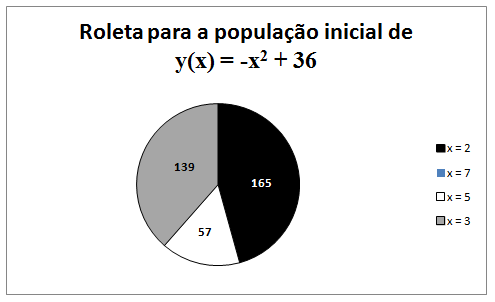
\includegraphics[width=13cm]{figs/ga/roleta_viciada.png}
		\end{center}
		\caption{\label{figRoleta}Roleta criada a partir dos dados da tabela \ref{tabSumFitness}. Note que o indivíduo x = 7 foi descartado porque sua avaliação foi um número menor do que zero.}
	\end{figure}
	
	Mas como implementar tal roleta? Um exemplo em Linguagem C encontra-se na figura \ref{figCodRoleta}. Na linha 226 um \textit{\texttt{for}} é definido de modo que as suas instruções sejam executadas \textit{\texttt{numindividuos}} vezes. Dessa maneira, a população de indivíduos mantêm-se fixa, e podemos trabalhar com vetores constantes. A próxima linha de código armazena em \textit{\texttt{vlrRoleta}} um número aleatório entre 0 e a soma das notas de todos os indivíduos (\textit{\texttt{sumFitness}}). Essa soma também é exibida na tabela \ref{tabSumFitness}. A variável \textit{\texttt{iSelecionado}} armazenará o índice do indivíduo selecionado.
	
	No laço \textit{\texttt{do ... while}} a roleta começa de fato a girar. A partir do primeiro indivíduo, somamos o \textit{fitness} de cada um em \textit{\texttt{sumFitness}}. Quando essa variável atingir um valor maior do que \textit{\texttt{vlrRoleta}}, o indivíduo com índice \textit{\texttt{iSelecionado}} na geração atual será transferido para a posição \textit{\texttt{iIndividuo}} da próxima geração (linha 238 da figura \ref{figCodRoleta}). 
	
	Apesar do caráter randômico do método, ele prevê, estatisticamente, que a quantidade de vezes que um cromossomo aparecerá na próxima geração é proporcional à sua nota. Portanto, não despreza completamente os indivíduos com menor \textit{fitness}, ao mesmo tempo que privilegia os mais aptos.

	\begin{figure}[htp]
		\begin{center}
			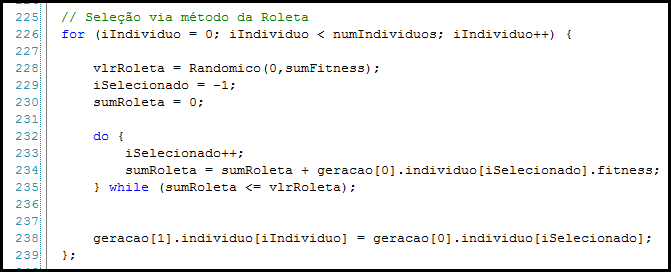
\includegraphics[width=13cm]{figs/ga/CodigoRoleta.png}
		\end{center}
		\caption{\label{figCodRoleta}Exemplo de código em Linguagem C para o método da Roleta.}
	\end{figure}
	
	\subsubsection{Seleção por torneio}
	
	Utilizada no mestrado porque o paralelismo é direto.
	
	\subsubsection{Exemplo: máximo da função $f(x) = -x^2 + 36$}
	
	Usaremos os dados da tabela \ref{tabSumFitness} para montar a roleta da figura \ref{figRoleta} e mostrar, passo a passo, o funcionamento do método.
	
	Como temos quatro indivíduos na população,
	
	$$
	numindividuos = 4.
	$$

	Devemos obter um número aleatrório entre 0 e 70 (soma dos fitness). Imagine que esse primeiro número tenha sido 65:
	
	$$
	vlrRoleta = 65.
	$$
	
	Entramos no \textit{\texttt{for}} e \textit{\texttt{iSelecionado}} é inicializada com -1:
	
	$$
	iSelecionado = -1.
	$$
	
	Já dentro do laço \textbf{\texttt{do ... while}}O primeiro indivíduo na geração é o $x = 2$, com \textit{fitness} igual a 32. Então \textit{\texttt{sumRoleta}} passa a ser também 32, mas continua menor do que \textit{\texttt{vlrRoleta}}:
	
	$$
		sumRoleta = 32 < vlrRoleta = 65.
	$$
	
	Ainda não é possível sair do laço \textit{\texttt{do ... while}}, e os passos são repetidos para o segundo indivíduo, $x = 7$. Entretanto, esse cromossomo obteve nota nula na função de avaliação, fazendo com que o valor de \textit{\texttt{sumRoleta}} não seja alterado pela soma da linha 234 (figura \ref{figCodRoleta}).
	
	O terceiro cromossomo possui nota 11, fazendo com que ainda permaneçamos dentro do laço:
	
	$$
		sumRoleta = 43 < vlrRoleta = 65.
	$$
	
	Chegamos ao último indivíduo da população. Seu \textit{fitness} é 27, permitindo a seleção:
	
	$$
		sumRoleta = 70 > vlrRoleta = 65.
	$$
	
	Na tabela \ref{tabRoletaManual} encontra-se uma comparação entre a geração inicial e final após a seleção via método da roleta. Os valores de \textit{\texttt{vlrRoleta}} foram obtidos utilizando a função \texttt{ALEATÓRIOENTRE} do Microsoft Excel.
	
\begin{table}[htp]
	\caption{\label{tabRoletaManual}Valores obtidos aleatoriamente para \textit{\texttt{vlrRoleta}} e os respectivos indivíduos selecionados. Note que o cromosso com \textit{fitness} zero foi eliminado e o \textit{fitness} médio aumentou.}
	\begin{center}
		\begin{tabular}{c|c|c|c|c}
			\hline
			\multicolumn{2}{c|}{\textbf{Geração inicial}} & \textbf{Roleta}& \multicolumn{2}{c}{\textbf{Geração final}}  \\
			\hline
			x 					& \textit{fitness} (n)	& vlrRoleta						& x						& \textit{fitness} (n)	\\
			\hline
			2 					& 32										& 65 									& 3						&	27   \\
			7 					& 0 										& 27 									& 2						&	32\\
			5 					& 11										& 70 									& 3						&	27\\	
			3 					& 27										& 41 									& 5						&	11\\
			\hline
			\multicolumn{2}{c|}{$<n>$ = 17,5} & - & \multicolumn{2}{c}{$<n>$ = 24,25}  \\
			\hline
		\end{tabular}
	\end{center}
\end{table}
	
	Dois fatos interessantes aconteceram. O indivíduo com \textit{fitness} zero foi eliminado conforme o esperado. Ele não ocupou espaço na roleta e, obviamente, não poderia participar do processo de seleção. Além disso, o \textit{fitness} médio ($<n>$) da nova população é superior ao da anterior, indicando que a Seleção cumpriu o seu papel em manter os mais aptos.
	
	
	\subsection{\label{crossover}Reprodução (\textit{Crossover})}

	A Reprodução consiste em combinarmos a informação genética de dois cromossomos da população e gerar um ou mais descendentes, até que o número de indivíduos da nova população seja atingido. Uma maneira simples é através do \textbf{\textit{Crossover} de ponto único} (figura \ref{figCrossOver}).
	
	\begin{figure}[htp]
		\begin{center}
			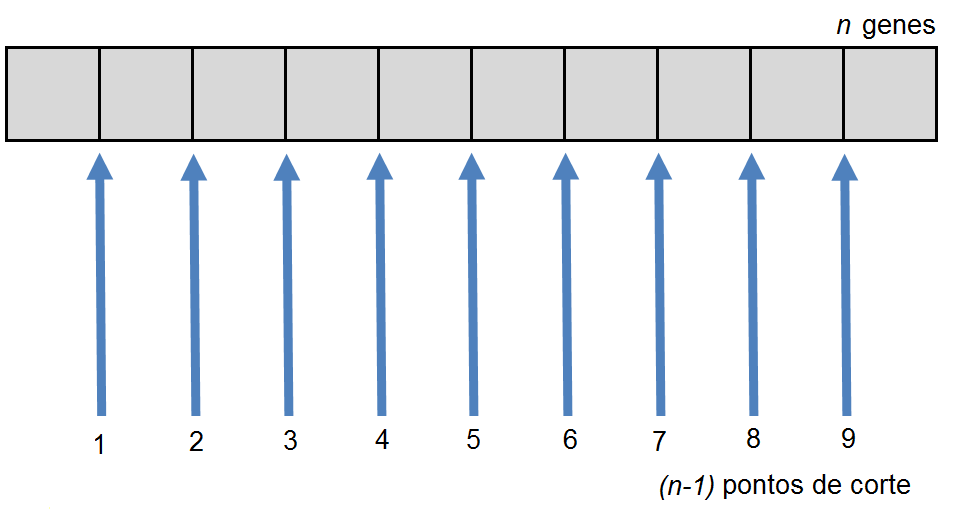
\includegraphics[width=6cm]{figs/ga/PontosCorte.png}
			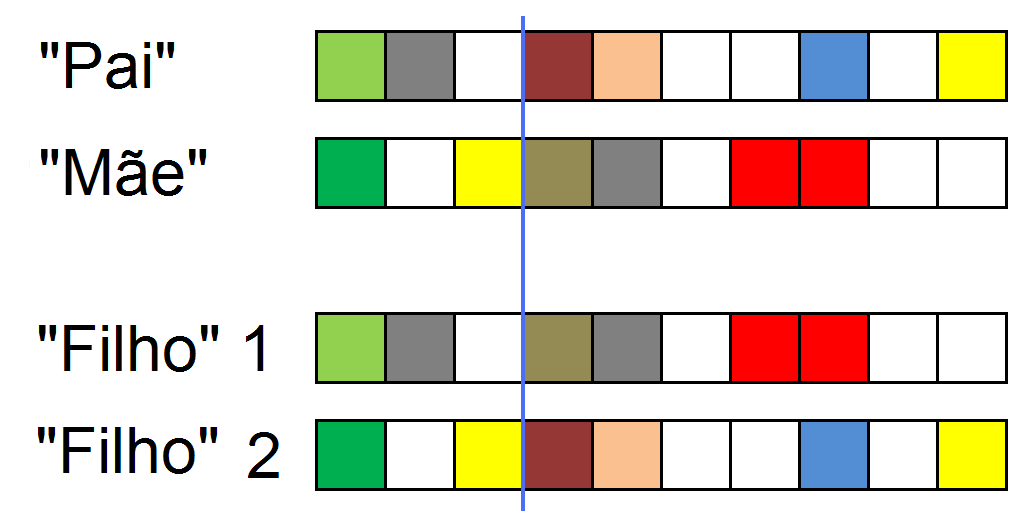
\includegraphics[width=6cm]{figs/ga/CrossOver.png}
		\end{center}
		\caption{\label{figCrossOver}Definição de Ponto de \textit{Corte} e o \textit{Crossover} de ponto único. Com esse operador conseguimos gerar até dois filhos para cada par de pais.}
	\end{figure}
	
	O primeiro passo é escolher dois cromossomos que farão o papel dos pais. Qualquer critério pode ser usado para compor esse par, como indivíduos que são diferentes geneticamente, ou agrupando os melhores e os piores separadamente. Porém, a escolha aleatória é a utilizada na maioria dos livros e aplicações, e, dada a sua simplicidade, será ela a abordada aqui. Tendo os pais em mãos, obtemos também aleatoriamente o ponto de corte, e estamos prontos para a reprodução (figura \ref{figCrossOver}). 
	
	Entretanto, voltando à Natureza, sabemos que a reprodução não acontece necessariamente sempre, e o nosso algoritmo deve contemplar esse efeito. Fazemos isso através de uma probabilidade $p_c$ associada à ocorrência do \textit{Crossover}. Digamos que $p_c = 70\%$. Após escolhidos os pais e o ponto de corte, sorteamos um número $p_{aux}$ entre $0$ e $1$ e, se $p_{aux} <= p_c$, o \textit{Crossover} acontece.
	
	Esse processo deve ser repetido até que o número de indivíduos desejado seja atingido. Nas figuras \ref{figCodLoopCrossOver} e \ref{figCodCrossOver} há um exemplo de código.
	
	\subsubsection{Exemplo: crossover para $f(x) = -x^2 + 36$}
	
	Para que o funcionamento do operador \textit{crossover} fique claro, faremos uma execução manual do código contido na figura \ref{figCodLoopCrossOver}. Os indivíduos que utilizaremos serão aqueles selecionados pela Roleta, presentes na tabela \ref{tabRoletaManual}. Ao final teremos quatro indivíduos provenientes de oito pares de cromossomos.
	
	Entrentando, antes de continuarmos, explicaremos o algoritmo.	A segunda linha, 248, inicializa a variável \textit{\texttt{flagCrossOver}} com zero, ou \texttt{falso} na linguagem C. A função dela é garantir que em todas as iterações do laço \textit{\texttt{for}} sairemos com um descendente.
	
	Entramos no \textit{\texttt{while}} e chamamos a função \textit{\texttt{GeraPontoDeCorte()}}, cujo trabalho é definir o ponto de corte e armazená-lo em uma variável global. Conforme pode ser visto na figura \ref{figCodCrossOver}, essa variável (\textit{\texttt{PontoDeCorte}}) é utilizada na função \textit{\texttt{CrossOver()}}.
	
	Cada elemento do vetor \textit{\texttt{geracao}} (linhas 251 e 252) armazena uma população com um número fixo de indivíduos, definida em \textit{\texttt{numindividuos}}. Então, para obter um cromossomo aleatoriamente, geramos, através da função \textit{\texttt{Randomico()}}, um valor entre zero e (\textit{\texttt{numindividuos}} - 1). Esse número será a posição do indivíduo escolhido dentro da geração. 	As variáveis \textit{\texttt{indPai}} e \textit{\texttt{indMae}} receberão os dois indivíduos. 
	
	Em \textit{\texttt{probAux}} guardamos um valor entre 0 e 1, obtido novamente de maneira aleatória. Se ele for menor ou igual a \textit{\texttt{probCrossOver}} (probabilidade de ocorrer a Reprodução), os indivíduos \textit{\texttt{indPai}} e \textit{\texttt{indMae}} gerarão um filho, que será armazenado na posição \textit{\texttt{iIndividuo}} da \textit{\texttt{geracao\_auxiliar}}. A \textit{\texttt{flagCrossOver}} recebe \textit{\texttt{verdadeiro}}, indicando que temos um descendente e podemos sair do \textit{\texttt{while}}.
	
	Voltemos à execução manual do nosso exemplo. Começamos definindo que a probabilidade de ocorrência da Reprodução será de 70\%\footnote{Não há um valor ótimo e absoluto para $p_c$. Para cada caso deve-se ajustar esse parâmetro e verificar a qualidade das soluções. Podemos afirmar apenas que $p_c$ deve ser alta, entre 70\% e 100\%.}:
	
	$$
		probCrossOver = 0,7.
	$$	
	
	Através da tabela \ref{tabRoletaManual} lembramos que 
	
	$$
		numindividuos = 4.
	$$
	
	Ao entrar no \textit{\texttt{for}} a \textit{\texttt{flagCrossOver}} recebe \textit{\texttt{falso}}:
	
	$$
		flagCrossOver = 0.
	$$

	Assim que chegamos ao \textit{\texttt{while}} a função \textit{\texttt{GeraPontoDeCorte()}} é executada. Como a nossa representação cromossomial possui três genes, há apenas dois pontos de corte possíveis (figura \ref{figCrossOver}). Digamos que a função escolha
	
	$$
		PontoDeCorte = 1,
	$$
	e que
	
	$$
		probAux = 0,86.
	$$
	
	Para esse caso, a condição \textit{\texttt{probAux <= probCrossOver}} é falsa, obviamente não entramos no \textit{\texttt{if}} e voltamos ao início do \textit{\texttt{while}}.
	
	Entretanto, suponha que agora os seguintes valores tenham sido obtidos:
	
	$$
		PontoDeCorte = 1 \mbox{  e  } probAux = 0,65.
	$$
	
	Na linha 251 \textit{\texttt{Randomico(0, numindividuos)}} retorna 0, e isso significa que \textit{\texttt{indPai}} recebeu $x = 3 = 011$:
	
	$$
		indPai = 011.
	$$
	
	Em seguida, \textit{\texttt{Randomico(0, numindividuos)}} retorna 3\footnote{Lembre-se que na linguagem C o primeiro elemento de um vetor possui índice \textit{i} = 0. Por isso o número 3 retornou o quarto elemento.}, e isso implica
	
	$$
		indMae = 101.
	$$
	
	\begin{figure}[htp]
		\begin{center}
			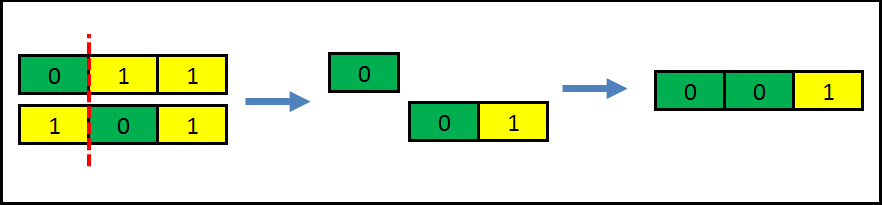
\includegraphics[width=13cm]{figs/ga/exemplo_crossover.png}
		\end{center}
		\caption{\label{figExemploCrossOver} Exemplo do \textit{crossover} entre os indivíduos 011 e 101 para o primeiro ponto de corte.}
	\end{figure}
	
	O resultado da reprodução, veja a figura \ref{figExemploCrossOver}, é armazenado na primeira posição da \textit{\texttt{geracao\_auxiliar}}:
	
	$$
		geracao\_auxiliar[0] = 001.
	$$
	
	Vamos refletir um pouco sobre esse resultado. Na geração atual (\textit{Geração Final} na tabela \ref{tabRoletaManual}) o indivíduo com melhor \textit{fitness} é o $x = 2$, enquanto $x = 5$ possui a pior nota e $x = 3$ obteve uma avaliação intermediária. Por causa do caráter completamente aleatório do algoritmo, o melhor indivíduo não foi selecionado para gerar descendentes nessa reprodução. Poderíamos supor, num primeiro momento, que esse não tenha sido o melhor caminho. Entretando, o resultado do \textit{crossover} entre $x = 5$ e $x = 3$ gerou um indivíduo com o maior \textit{fitness} desde a geração inicial! Usando $x = 1$ na $f(x)$ chegamos a $f_c(1) = 35$, maior do que o $f(2) = 32$.
	
\begin{table}[htp]
	\caption{\label{tabCrossoverManual}Geração antes e depois do \textit{Crossover}. O melhor indivíduo dos descendentes possui o melhor \textit{fitness} entre todas as gerações anteriores. Além disso, o \textit{fitness} médio ($<n>$) também aumentou.}
	\begin{center}
		\begin{tabular}{c|c|c|c}
			\hline
			\multicolumn{2}{c|}{\textbf{Geração Selecionada}} &  \multicolumn{2}{c}{\textbf{Descendentes}}  \\
			\hline
			x 					& \textit{fitness} (n)	& x						& \textit{fitness} (n)	\\
			\hline
			3 					& 27										& 1						&	35 \\
			2 					& 32 										& 5						&	11 \\
			3 					& 27										& 3						&	27 \\	
			5 					& 11										& 3						&	27\\
			\hline
			\multicolumn{2}{c|}{$<n>$ = 24,25} & \multicolumn{2}{c}{$<n>$ = 25,00}  \\
			\hline
		\end{tabular}
	\end{center}
\end{table}
	
	A tabela \ref{tabCrossoverManual} apresenta os dados do nosso processo de Reprodução feito manualmente. É interessante notar que, apesar dessa nova geração ter perdido o indivíduo $x = 2$, a maior avaliação da população anterior, o \textit{fitness} médio aumentou. Não só isso, mas também o melhor cromossomo tem uma nota maior do que todos os indivíduos anteriores. 
	
	Apesar de simples, o exemplo acima exibiu o papel fundamental do \textit{Crossover} na busca pelas melhores soluções. Na próxima seção mostraremos como funciona a Mutação, essencial para a variabilidade genética. 
	
	\begin{figure}[htp]
		\begin{center}
			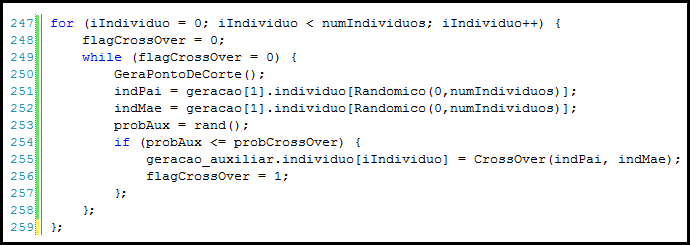
\includegraphics[width=13cm]{figs/ga/CodigoLoopCrossOver.png}
		\end{center}
		\caption{\label{figCodLoopCrossOver} Código para a Reprodução. Nesse exemplo o algoritmo gera apenas um descendente. Detalhes da função \texttt{CrossOver()} estão na figura \ref{figCodCrossOver}.}
	\end{figure}

\begin{figure}[htp]
		\begin{center}
			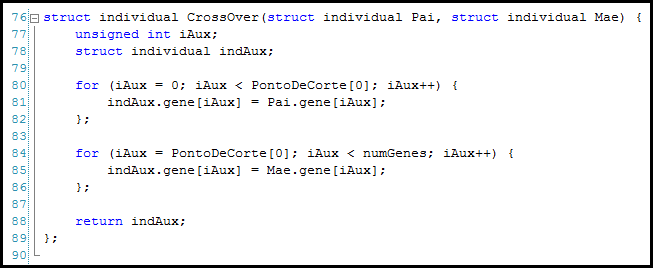
\includegraphics[width=13cm]{figs/ga/CodigoCrossOver.png}
		\end{center}
		\caption{\label{figCodCrossOver}Detalhes da função \texttt{CrossOver()}.}
	\end{figure}
	
	\subsection{\label{mutacao}Mutação}
		
	Chegamos à última operação de um algoritmo genético, a Mutação. Assim como no \textit{Crossover}, existe uma probabilidade $p_m$ associada ao acontecimento da Mutação. Porém, nesse momento, não operaremos sobre um par de cromossomos, mas na estrutura interna de cada cromosso: os genes.
	
	Se nossos indivíduos possuem dez genes, para cada um dos dez \textit{locus} testamos a condição $p_{aux} <= p_m$, onde $p_{aux}$ é um valor entre zero e um, escolhido aleatoriamente. Caso a desigualdade seja verdadeira, invertemos o \textit{bit} daquela posição e partimos para o próximo \textit{locus}.
	
	Seguindo com o exemplo da seção anterior, a população atual, depois da Seleção e do \textit{Crossover}, possui o melhor indivíduo comparado com os anteriores, além do \textit{fitness} médio também ter crescido (tabela \ref{tabCrossoverManual} na página \pageref{tabCrossoverManual}). Na tabela \ref{tabPopAntesMutacao} listamos esses indivíduos e a sua representação cromossomial.
	
	\begin{table}[htp]
 		\caption{\label{tabPopAntesMutacao}Representação cromossomial para os indivíduos que passaram pela Seleção e pelo \textit{Crossover}.}
 		\begin{center}
  		\begin{tabular}{c|c}
   			\hline
   			\textbf{x (decimal)}  & \textbf{x (representação binária)} \\
   			\hline
   			1 & 001 \\
   			5 & 101 \\ 
   			3 & 011 \\
   			3 & 011 \\
   			\hline
   		\end{tabular}
 		\end{center}
	\end{table}
	
	Do ponto de vista da informação genética, o indivíduo que mais se aproxima de $x = 0 = 000$, a solução ideal, é o $x = 1 = 001$. Portanto, bastaria evoluir essa população e, em algum momento, obteríamos a melhor solução, certo? Errado.
	
	Nenhum indivíduo possui um zero na última posição. Então, mesmo fazendo todas as combinações possíveis entre os cromossomos, nunca chegaríamos ao indivíduo $x = 0$. O único que possuía tal característica era o $x = 2$, presente na população inicial mas ``extinto'' ao longo da evolução.
	
	É aí que entra a Mutação: ainda que baixa, geralmente em torno de 1\%, há uma chance do último \textit{bit} de algum indivíduo sofrer mutação e ser alterado para zero. E esse é um dos pontos que torna a Mutação tão importante: ela insere uma nova informação genética que, ou foi perdida, ou não estava presente na população inicial (Heurística Exploratória).
	
	\begin{figure}[htp]
		\begin{center}
			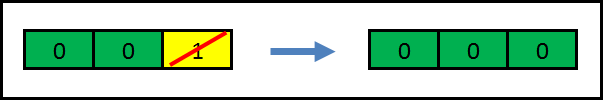
\includegraphics[width=13cm]{figs/ga/Mutacao.png}
		\end{center}
		\caption{\label{figMutacao}Representação gráfica de uma mutação. Nesse exemplo a mutação no último \textit{bit} levou à solução ótima para o máximo da função $f(x) -x^2 + 36$.}
	\end{figure}
	
	Obviamente, existe a possibilidade de bons esquemas serem destruídos com a mudança em algum ``\textit{bit} errado''. Mesmo assim, essa chance é equivalente à probabilidade de transformarmos um péssimo esquema em um excelente espaço de soluções. Nessa linha, a Mutação é a responsável por manter a diversidade e evitar a Convergência Genética (seção \ref{ExemploVariabilidade}).
	
	Qual deve ser o valor de $p_m$ para uma Mutação eficiente? Não há uma resposta absoluta. Muitos pesquisadores e usuários dos GAs utilizam valores entre 0,5\% e 1\%, simplesmente porque nos primeiros trabalhos bons resultados foram obtidos com eles. Sabe-se que há um valor ideal, mas ele é diferente para cada problema e para cada representação cromossomial.
	
	Apesar disso, há um consenso de que o valor de $p_m$ deve ser pequeno, bem menor do que $p_c$. Em parte porque na genética natural essa probabilidade é de fato pequena, mas principalmente, no contexto da computação, porque valores grandes fariam com que a busca por soluções se comportasse de maneira semelhante ao \textit{Random Walk}.
	
	Partindo para o lado prático, o código para implementar a mutação é mais simples, e um exemplo encontra-se na figura \ref{figCodMutacao}. Na linha 281 um determinado indivíduo recebe ele próprio após o operador Mutação. Não há \textit{\texttt{if}} ou outra condição, ou seja, aplicamos o operador em todos os indivíduos da população.
	
	\begin{figure}[htp]
		\begin{center}
			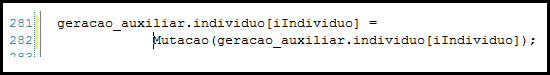
\includegraphics[width=13cm]{figs/ga/CodigoMutacao.png}
			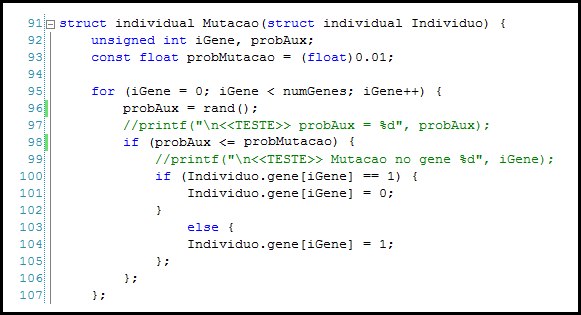
\includegraphics[width=13cm]{figs/ga/CodigoMutacaoFunc.png}
		\end{center}
		\caption{\label{figCodMutacao}Exemplo de código para o operador Mutação.}
	\end{figure}
		
	Mas, afinal, onde está a probabilidade $p_m$? Lembre-se que a mutação, caso aconteça, deve ocorrer isoladamente em cada gene. Por isso usamos $p_m$ dentro da função \textit{\texttt{Mutacao()}}. Ela recebe como parâmetro um indivíduo que possui um número de genes igual a \textit{\texttt{numGenes}}, uma constante definida de maneira global.
	
	Entramos em um \textit{\texttt{for}} que irá varrer todos os genes do \textit{\texttt{Individuo}} e, para cada um, faz o teste $p_{aux} <= p_m$. Se a condição retornar \textit{\texttt{verdadeiro}}, a Mutação é finalmente expressa como a inversão do \textit{bit} no \textit{locus} atual.
	
	Depois que todos os indivíduos da população passarem pelo operador Mutação, o ciclo estará fechado. A nova geração está pronta para passar por todo o processo: Avaliação, Seleção, Reprodução e Mutação.
	
	\section{Considerações finais}
	
	A Teoria da Evolução de Darwin causou uma das principais revoluções na ciência. Seu impacto não está restrito à Biologia, e os Algoritmos Genéticos (GAs), um ramo da Computação Evolutiva, são um bom exemplo disso.
	
	Fortemente inspirado no processo de Seleção Natural, todo GA possui uma representação chamada Cromossomial, o equivalente ao DNA. A população de soluções é avaliada para verificar quais são as ruins, as boas e as melhores. As mais adequadas têm maior chance de se reproduzirem e perpetuar seus genes.
	
	Do ponto de vista da Inteligência Artificial, os GAs são aplicados com sucesso em vários problemas. Alguns exemplos, dentre muitos, são o reconhecimento de padrões em visão computacional, movimentação de membros em robótica, criação de ambimentes mais realistas em jogos e treinamento de redes neurais. 
	
	Estruturalmente todo GA é semelhante, facilitando a modularização do código. Gera-se a população inicial que é avaliada e, em seguida, ela passa pela Seleção, \textit{Crossover} e Mutação. Novos indivíduos são criados e, depois de algumas gerações, chegamos a uma população com um conjunto de boas soluções.
	
	Mesmo com boa aplicabilidade, os GAs devem ser utilizados com cuidado. Dada a natureza aleatória do método, não há garantia em geral de uma solução ótima seja encontrada e, por isso, algoritmos que levam à soluções exatas têm prioridade.
	
	Porém, problemas combinatoriais muito grandes, como os NP Completos, são um excelente campo de utilização. Além desses, os GAs são eficientes na otimização de problemas multiobjetivos, como escala de horários ou planejamento de logística e produção.



